\documentclass[12pt,a4paper]{article}
\usepackage[utf8]{inputenc}
\usepackage{amsmath}
\usepackage{amsfonts}
\usepackage{amssymb}
\usepackage{graphicx}
\usepackage{color}
\usepackage{multirow}
\usepackage{array}
\usepackage{booktabs}


\author{Jonathan Leblanc, Guillaume Pelletier}
\title{American-Style Options using Backward Differentiation Formula}

\newcommand{\ninf}[1]{\left\| {#1} \right\|_\infty}
\newcommand{\abs}[1]{\left\vert {#1} \right\vert}
\newcommand{\reel}{\mathbb{R}}
\newcommand{\atan}{\text{atan}}
\newcommand{\pd}[2]{\frac{\partial {#1}}{\partial {#2}}}
\newcommand{\pdd}[2]{\frac{\partial^2 {#1}}{\partial {#2}^2}}
\newcommand{\pdc}[3]{\frac{\partial^2 {#1}}{\partial {#2} \partial {#3}}}

\begin{document}
\maketitle
\newpage

\section{Introduction}

The aim of this project is to use Backward Differentiation Formula (BDF) to solve non-linear diffusion equations with an obstacle term, in particular American-style options. We aim to reproduce numerical results from \cite{Boka} and \cite{Oosterlee}.

We mainly focus on partial differential equation (PDE) with an obstacle term of the following form,
\begin{align}
	\min \left( u_t + \mathcal{A} u, u - \phi(x) \right) = 0,& \quad t \in (0,T), x \in \Omega, \label{eq-obstacle}\\
	u(0, x) = u_0(x),& \quad x \in \Omega \label{eq-obstacle_initcond}
\end{align}
with $\mathcal{A}u := -\frac{1}{2} \sigma^2(t,x) u_{xx} + b(t,x) u_x + r(t,x) u$, and $\sigma$, $b$ and $r$ assumed to be regular functions.

In this report, we first present BDF implicit schemes and examine stability results on an american-style put option. We revisit two types of Crank-Nicolson schemes to compare the stability of the schemes, especially for high CFL\footnote{See later. TO BE UPDATED} numbers.

In section 2 we look at several numerical examples where we have explicit solutions. Compared to first section, we are abble to have finer study of the convergence near the singular region. Models examined are (\ref{eq-obstacle}), but we also have a look at one and two-dimensionnal problems based on Laplace operator.

\section{Implicit BDF Obstacle Schemes}

	\subsection{Backward Differentiation Formula}

Our motivation for using BDF schemes is to unconditionally improve the consistency in time. We will see that with a particular treatment for the obstacle term, a Crank-Nicolson scheme yields second-order time consistency if the CFL condition holds. We aim do better and for that we analyse schemes up to step 3, that is BDF-2 and BDF-3, even though higher orders exist (up to 6).

Let us consider a domain $\Omega = [X_{min}, X_{max}]$ and a uniform mesh with $J$ points inside, $x_j = X_{min} + jh$ for $j = 0, \dots, J+1$, where $h = \frac{X_{max} - X_{min}}{J+1}$. Moreover, $N \geq 1$ the number of time points in $[0,T]$, we define $t_n = n \tau$ for $n = 0, \dots N$, with $\tau = \frac{T}{N}$.

We consider the obstacle problem (\ref{eq-obstacle}) complemented by boundary conditions of Dirichlet type, $\forall t \in (0,T)$
\begin{align} 
	u(t, X_{min}) = u_l(t), \label{eq-obstacle_ul}\\
	u(t, X_{max}) = u_r(t). \label{eq-obstacle_ur}
\end{align}
Denoting by $u_j^n$ an approximation of $u(t_n, x_j)$, we use a centered finite difference aproximation for the operator $\mathcal{A} u$. When $\mathcal{A}$ does not depend on time -- which is the case for Black-Scholes' equation -- we have the approximation,
\begin{align*}
	(\mathcal{A} u)(t_n, x_j) &\simeq - \frac{\sigma^2(x_j)}{2} \left( \frac{u_{j+1}^n - 2u_j^n + u_{j-1}^n}{h^2} \right) + b(x_j) \frac{u_{j+1}^n - u_{j-1}^n}{2h} + r(x_j) u_j^n \\
	& = \left( A u^n + q(t_n) \right)_j.
\end{align*}
The matrix $A$ is tridiagonal with $A = \text{tridiag} \left( -\alpha_j-\beta_j, 2\alpha_j + \gamma_j, -\alpha_j+\beta_j \right)$ where $\alpha_j = \frac{\sigma^2(x_j)}{2h^2}$, $\beta_j = \frac{b(x_j)}{2h}$, $\gamma_j = r(x_j)$, and $u^n = (u_1^n, \dots, u_J^n)^T$ and boundary conditions dealt by $q(t_n) = \left( -(\alpha_1+\beta_1) u_l(t_n), 0 \dots 0, (-\alpha_J+\beta_J) u_r(t_n) \right)^T$.

We can now introduce the BDF-2 scheme for the obstacle equation (\ref{eq-obstacle}) as
\begin{align}
	\mathcal{S}_j^{n+1} (u) := \min\left( \frac{3 u_j^{n+1} - 4 u_j^n + u_j^{n-1}}{2 \tau} + (A u^{n+1} + q(t_{n+1}))_j, u_j^{n+1} - g_j \right) = 0 \label{eq-BDF2}
\end{align}
for $n=0,\dots,N$, $j=1,\dots,J$. We have denoted the obstacle value $g_j := \phi(x_j)$. Using Taylor's theorem, we demonstrate that the scheme is second order consistent in time (and space), and
\begin{align*}
	\mathcal{S}^{n+1} (v) = & \min (v_t + \mathcal{A}v, v-\phi)(t_{n+1}, x_j) \\ 
		& \quad + O(\tau^2 \ninf{v_{3t}}) + O(h^2 (\ninf{v_{3x}} + \ninf{v_{4x}})),
\end{align*}
when $v$ is regular (see Appendix for proof). 

Another equivalent way of writting the scheme (\ref{eq-BDF2}) is
\begin{align}
	\mathcal{S}^{n+1} (u) = \min\left( (I_d +\frac{3}{2} \tau A) u^{n+1} - \frac{4}{3} u^n + \frac{1}{3} u^{n-1} + \frac{2}{3} \tau q(t_{n+1})), u^{n+1} - g \right) = 0, \label{eq-BDF2_bis}
\end{align}
with $g = (g_1, \dots, g_J)^T$.

Using the same arguments, we derive the BDF third order implicit obstacle scheme (BDF-3),
\begin{align}
	\mathcal{S}_j^{n+1} (u) := \min\bigg( &\frac{\frac{11}{6} u_j^{n+1} - 3 u_j^n + \frac{3}{2} u_j^{n-1} - \frac{1}{3} u_j^{n-2}}{\tau} \nonumber\\
	& \quad + (A u^{n+1} + q(t_{n+1}))_j, u_j^{n+1} - g_j \bigg) = 0 \label{eq-BDF3}
\end{align}
for $n=0,\dots,N$, $j=1,\dots,J$, when $\mathcal{A}$ does not depend on time. As before, we have the equivalent scheme
\begin{align}
	\mathcal{S}^{n+1} (u) = \min\bigg( & (11 I_d + 6 \tau A) u^{n+1} - 18 u^n + 9 u^{n-1} \nonumber\\ 
	& \quad - 2 u^{n-2} + 6 \tau q(t_{n+1})), u^{n+1} - g \bigg) = 0. \label{eq-BDF3_bis}
\end{align}
This time, Taylor's theorem give us a third order consistency in time (see Appendix for proof), thus for $v$ regular,
\begin{align*}
	\mathcal{S}^{n+1} (v) = & \min (v_t + \mathcal{A}v, v-\phi)(t_{n+1}, x_j) \\ 
		& \quad + O(\tau^3 \ninf{v_{4t}}) + O(h^2 (\ninf{v_{3x}} + \ninf{v_{4x}})),
\end{align*}

To solve both non-linear schemes (\ref{eq-BDF2_bis}) and (\ref{eq-BDF3_bis}), we use a semi-smooth Newton's method. This algorithm is very efficient in solving obstacle problem of the form
\begin{align}
	\min (Bx - b, x-g) = 0, \quad x \in \reel^J. \label{eq-Newton}
\end{align}
As soon as $B$ is an $M$-matrix, it was shown in \cite{MR2551155}, that exact convergence happens in less that $(J+1)$ steps.

	\subsection{Crank-Nicolson Schemes}

We focus on BDF schemes, but in order to challenge consistency and stability results, we need another scheme as reference : we choose Crank-Nicolson schemes. On purpose, we give only brief descriptions and explanations, and refer to \cite{Boka} for more details and proofs.

We give a first naive Crank-Nicolson (CN) scheme of the obstacle problem (\ref{eq-obstacle}),
\begin{align}
\mathcal{S}^{1,n} := \min \left( \frac{u^{n+1}-u^n}{\tau} + \frac{1}{2} (Au^{n+1} + Au^{n}) + q(t_{n+1/2}), u^{n+1} - \phi \right) = 0. \label{eq-CN1}
\end{align}
It is well known that CN schemes have second order consistency in time and space. However, the second order consistency happens only at times $t_{n+\frac{1}{2}}$, while the obstacle is evaluated at time $t_n$. Hence, scheme (\ref{eq-CN1}) is only one order consistent in time,
\begin{align*}
\mathcal{S}_j^{1,n} (v) = \min( v_t + \mathcal{A}v, v - \varphi) (t_{n+\frac{1}{2}}, x_j) + O(\tau + h^2).
\end{align*}

An ingenious way of overcomming this weak time consistency is to use the following equivalent formulation of the obstacle problem (\ref{eq-obstacle}),
\begin{align}
	\min( -u_t + \mathcal{A}u, -u_t) &= 0 \; &t &\in (0,T), x \in \Omega, \label{eq-obstacle_reform}\\
	u(0, x) &= u_0(x), \; & x &\in \Omega \nonumber.
\end{align}
Using a centered finite difference for $v_t$ in the obstacle term, the CN scheme for (\ref{eq-obstacle_reform}) is
\begin{align}
\mathcal{S}^{2,n} := \min \left( \frac{u^{n+1}-u^n}{\tau} + \frac{1}{2} (Au^{n+1} + Au^{n}) + q(t_{n+1/2}), u^{n+1} - u^{n} \right) = 0. \label{eq-CN2}
\end{align}
Unlike the naive CN scheme, the obstacle term of (\ref{eq-CN2}) is second order time consistent at time $t_{n+\frac{1}{2}}$, hence,
\begin{align*}
\mathcal{S}_j^{2,n} (v) = \min( v_t + \mathcal{A}v, v - \varphi) (t_{n+\frac{1}{2}}, x_j) + O(\tau^2 + h^2).
\end{align*}

		\subsection{Error Estimate for the BDF-2 Implicit Scheme}

On étudiera aussi la preuve de la stabilité de la méthode [18].

		\subsection{Stability American-Style Put Option}

En particulier on tachera d’observer la convergence numérique d’ordre deux en temps et en espace, sans condition de type CFL dans le cas de BDF2.

	\section{Numerical results}

		\subsection{American-Style Put Option}

When pricing american-style put options in the first part, we did not know about the exact solution and estimated the erreur using a proxy which was computed using a very dense mesh\footnote{N=??? and J=???} and a BDF-2 scheme. In this section, we wish to have a finer estimation of the erreur, with particular attention near the singular point.

Let us consider the PDE of an american-style put option in the Black-Scholes model, and add a source term $f = f(t,x)$, thus 
\begin{align}
	\min \left( v_t - \frac{\lambda^2}{2} x^2 v_xx - r x v_x + r v, v - g(x) \right) = f(t,x), \label{eq-PDE_ameroption_source}
\end{align} 
with $g(x) := (K-x)^+$. It is well know that american-style put option price sticks to the payoff until a certain point $x_s(t) \in [0; K]$, with $x_s$ a decreasing function, and then gets strickly greater. Thus, we define
\begin{align*}
	x_s(t) := K - c_0 t,  \quad t \in [0,T]
\end{align*}
with $K-c_0T \in (0, K)$, and $X_{max}$, $0<K<X_{max}$, $c_0>0$ and $T>0$ given constants. So that the explicit functions $v(t,x)$ looks like a price, it must satisfy,
\begin{small}
\begin{enumerate}
	\item $v(t,x) = g(x)$ for $x \leq x_s(t)$,
	\item $v(t,x) > g(x)$, for $x > x_s(t)$,
	\item $v$ is at least $\mathcal{C}^1$ on $[0, X_{max}]$,
	\item $v(t,X_{max}) = 0$.
\end{enumerate}
\end{small}

Two functions $v$ are examined in \cite{Boka}, of which
\begin{align}
	v(t,x) = \left\lbrace \begin{array}{ll}
	g(x), \quad & \forall x < x_s(t), \\
	g(x_s(t)) - \frac{x - x_s(t)}{1 - (x - x_s(t))/C(t) }, \quad & \text{otherwise}.	
	\end{array} \right. \label{eq-explicit_sol_ameroption1}
\end{align}
where $C(t,0)$ is defined as to meet condition 4, thus
\begin{align*}
	C(t) := \left( \frac{1}{X_{max} - x_s(t)} - \frac{1}{g(x_s(t))} \right)^{-1}.
\end{align*}
The second explicit function defined is
\begin{align}
	v(t,x) = \left\lbrace \begin{array}{ll}
	g(x), \quad & \forall x < x_s(t), \\
	g(x_s(t)) - C(t) \atan \left( \frac{x - x_s(t)}{C(t)} \right), \quad & \text{otherwise}.	
	\end{array} \right. \label{eq-explicit_sol_ameroption2}
\end{align}
where $C(t,0)$ is defined\footnote{see \cite{Boka} for details on the two fixed-point methods used to compute $C(t)$} as to satisfy condition 4.

To solve (\ref{eq-PDE_ameroption_source}) with source function computed with (\ref{eq-explicit_sol_ameroption1}) or (\ref{eq-explicit_sol_ameroption2}), we use the semi-smooth Newton method. The algorithm solve very efficiently $\min (Bx - b, x-g) = 0$, thus with BDF-2 scheme on (\ref{eq-explicit_sol_ameroption1}) we end up with
\begin{align*}
	B &= I_d + \frac{2 \tau}{3} A, \\
	b &= \frac{4}{3} U^n - \frac{1}{3} U^{n-1} - \frac{2}{3} \tau q_{n+1} + \frac{2}{3} \tau f_{n+1} \\
	g &= g - f_{n+1}.
\end{align*}

		\subsection{Model problem based on Laplace Operator}

As in \cite{Oosterlee}, we consider the optimisation problem modelling elasto-plastic torsion of a cylindrical bar in a model region $\Omega = (-1,1) \times (-1,1)$. We added a partial derivation with respect to $t$ to test the BDF scheme, thus for all $t \in [0,T]$,
\begin{equation}
\label{eq-Laplace}
\begin{aligned}
	v_t + v_{ss} + v_{yy} &\leq C, & \quad x &\in \Omega, \\
	v &\leq d(x, \partial \Omega), & \quad x &\in \Omega, \\
	(v-d(x,\partial \Omega))(v_{ss} + v_{yy} - 2C) &= 0, \quad & x &\in \Omega, \\
	\text{with boudary cond.} \; v &= 0, \quad & x &\in \partial \Omega,
\end{aligned}
\end{equation}
where the $d(x, \partial \Omega)$-operator measures the distance from the grid point $x = (s,y)$ to the domain boundary $\partial \Omega$.

Just like for the american-style put option, we do not know about the exact solutions, and add a source term to construct explicit solutions. Moreover, we start by solving the problem in 1-dimension, thus (\ref{eq-Laplace}) reduces to
\begin{equation}
\label{eq-Laplace_1d}
\begin{aligned}
	\max(v_t + v_{ss} - C, v - d(x, \partial \Omega)) &= f(t,x), & \quad x &\in \Omega, \\
	\text{with boudary cond.} \; v &= 0, \quad & x &\in \partial \Omega.
\end{aligned}
\end{equation}
and $\Omega = [0,1]$.
We define $x_l(t) := -c_0 t$, $x_r(t) := c_0 t$ with $c_0 T < 1$, and $c_0>0$, $T>0$ fixed constants. The explicit solution $v$ must satisfy, for all $t \in [0,T]$,
\begin{small}
\begin{enumerate}
	\item $v(t,x) = d(x, \partial \Omega)$ for $x \in [-1, x_l(t)) \cap (x_r(t), 1]$,
	\item $v(t,x) < d(x, \partial \Omega)$, for $x < x_s(t)$,
	\item $v$ is at least $\mathcal{C}^1$ on $[-1, 1]$,
	\item $v(t,-1) = v(t,1) = 0$.
\end{enumerate}
\end{small}

From all these conditions, we derive the following parabola
\begin{align}
	v(t,x) = \left\lbrace \begin{array}{ll}
	d(x, \partial \Omega), \quad & \forall x \in [-1, x_l(t)) \cap (x_r(t), 1], \\
	d(x_r(t), \partial \Omega) + \frac{x_r(t)}{2} - \frac{x^2}{2 x_r(t)}, \quad & \text{otherwise}.	
	\end{array} \right. \label{eq-explicit_sol_ameroption2}
\end{align}

We fit a BDF-2 approximation for the first derivative $v_t$ and a centered finite difference aproximation for the second derivative $v_{ss}$. This leads us to the scheme
\begin{align*}
	S^{n+1}(u) := \max \bigg( &(I_d +\frac{2\tau}{3} A) u^{n+1} - \frac{4}{3} u^n + \frac{1}{3} u^{n-1} + \frac{2\tau}{3} (q_{n+1} - C - f^{n+1}), \\
	& \quad u^{n+1} - D - f^{n+1} \bigg) = 0
\end{align*} 
where $D = (d(x_1, \partial \Omega), \dots, d(x_J, \partial \Omega))^T$, $f^{n+1} = (f(t^{n+1},x_1), \dots, f(t^{n+1},x_J))^T$, $A = \text{tridiag} \left( \frac{1}{h^2},-\frac{2}{h^2},\frac{1}{h^2} \right)$, $q_{n+1} = \left( \frac{1}{h^2} x_l(t_{n+1}), 0 \dots 0, \frac{1}{h^2} x_r(t_{n+1}) \right)^T$ and $J$ the number of space points inside the mesh. This equation is solved using the usual\footnote{Notice the right-hand-side in the $\min$ is slightly different than the algorithm used in previous sections.} semi-smooth Newton's method for $\min(Bx - b, g - x) = 0$.

		\subsection{Heston Stochastic Volatility Model}

	In previous sections, we priced american-style put option in the basic Black-Scholes model, with constant volatility. Now, we consider the volatility to be stochastic using the Heston model. Let $(S_t)_{t \in [0,T]}$ the asset price and $(Y_t)_{t \in [0,T]}$ its variance process be defined by,
\begin{align}
	\frac{dS_t}{S_t} &= \mu dt + \sqrt{Y_t} dW^1_t, \\
	\frac{dY_t}{Y_t} &= \alpha (\beta - y) dt + \gamma dW^2_t,
\end{align}
where $W^1$, $W^2$ represent standard Brownian motion with correlation $\rho \in [-1, 1]$. The process $(Y_t)_{t \in [0,T]}$ is positive (provided that $\gamma^2 \leq 2 \alpha \beta$), mean-reverting with mean $\beta$ and rate governed by $\alpha$, and has volatility $\gamma$. 

Under this model, one can derive the following PDE for the value $u=u(x,y,t)$ of an option,
\begin{align}
	Lu := \pd{u}{t} - \mathcal{A}u = 0, \quad u(x,y,T) = g(x)\label{eq-EDPHeston}
\end{align}
where,
\begin{align}
	\mathcal{A}u = \frac{1}{2} \left( S_t^2 Y_t \pdd{u}{x} + 2 \rho \gamma Y_t S_t \pdc{u}{x}{y}+ \gamma^2 y \pdd{u}{y} \right) + r S_t \pd{u}{x} + \alpha (\beta - Y_t) \pd{u}{y} - ru, \label{eq-A_Heston}
\end{align}
and $g$ the payoff function.
We refer to \cite{Oosterlee,MR1628686} for the argument leading to (\ref{eq-EDPHeston}). For the put option, $g(x) = (E-x)^+$ and we use the same boudary conditions as \cite{Oosterlee}, that is Dirichlet conditions for $X_{min}=0$ and $Y_{min}=0$ of the form
\begin{equation}\label{eq-Heston_Dirichlet}
\begin{aligned}
	u(0, y, t) &= E e^{-r(T-t)}, \quad &\forall y &\geq 0, t \in [0,T], \\
	u(x, 0, t) &= (E-x)^+ e^{-r(T-t)}, \quad &\forall x &\geq 0, t \in [0,T], \\	
\end{aligned}
\end{equation}
and Neumann conditions at $S_{max}$ and $X_{max}$,
\begin{equation}\label{eq-Heston_Neumann}
\begin{aligned}
	\pd{u}{x}(X_{max}, y, t) &= 0, \quad &\forall y &\in [0,Y_{max}], t \in [0,T], \\
	\pd{u}{y}(x, Y_{max}, t) &= 0, \quad &\forall x &\in [0,X_{max}], t \in [0,T]. \\	
\end{aligned}
\end{equation}

As for the Black-Scholes model, one can derive the formulation for american-style put option,
\begin{equation} \label{eq-HestonObstacle}
\begin{aligned}
	\min \left( \pd{u}{t} + \mathcal{A}u, u - g(x) \right) &= 0, \\
	u(x, y, 0) &= g(x)
\end{aligned}
\end{equation}
with boundary conditions (\ref{eq-Heston_Dirichlet}) and (\ref{eq-Heston_Neumann}).

Let us consider a domain $\Omega = [X_{min}, X_{max}] \times [Y_{min}, Y_{max}]$ and a uniform mesh with $J$ points inside for $x$ and $K$ for $y$. We define $x_j = X_{min} + jh_x$ for $j = 0, \dots, J+1$, where $h_x = \frac{X_{max} - X_{min}}{J+1}$, and likewise $y_k = Y_{min} + kh_y$ for $k = 0, \dots, K+1$, where $h_x = \frac{Y_{max} - Y_{min}}{K+1}$. Moreover, $N \geq 1$ the number of time points in $[0,T]$, we define $t_n = n \tau$ for $n = 0, \dots N$, with $\tau = \frac{T}{N}$.

Denoting $u_{j,k}^n$ an approximation of $u(x_j,y_k,t_n)$, we consider a centered finite difference approximation for the operator $\mathcal{A}u$,
\begin{footnotesize}
\begin{align*}
	&(\mathcal{A}u)(x_j,y_k,t_n) \simeq \\
	&-\frac{1}{2} \bigg( x_j^2 y_k \frac{u_{j+1,k}^n - 2u_{j,k}^n + u_{j-1,k}^n}{h_x^2} 
	 +2 \rho \gamma y_k x_j \frac{u_{j+1,k+1}^n - u_{j+1,k-1}^n - u_{j-1,k+1}^n + u_{j-1,k-1}^n}{4 h_x h_y} \\ 
	&+ \gamma^2 y_k \frac{u_{j,k+1}^n - 2 u_{j,k}^n + u_{j,k-1}^n}{h_y^2} \bigg) - r x_j \frac{u_{j+1,k}^n-u_{j-1,k}^n}{2h_x} - \alpha (\beta - y_k) \frac{u_{j,k+1}^n - u_{j,k-1}^n}{2 h_y} + ru_{j,k}^n
\end{align*}
\end{footnotesize}
and a BDF-2 approximation for the first derivative $u_t$. Let us denote by $A u^n + q(t_n)$ the approximation of $\mathcal{A}u(.,.,t_n)$ on a given set of grid points, with $u^n = (u_{\bullet,1}^n,\dots,u_{\bullet,K}^n)^T$ and $u_{\bullet,k}^n = (u_{1,k}^n,\dots,u_{J,k}^n)^T$ and with given Dirichlet boudary conditions,
\begin{align*}
u_{0,k}^n = E e^{-r t_n}, \quad u_{j,0}^n = (E-x_j)^+ e^{-r t_n}, \quad k=1,\dots,K, \; j=1,\dots J.
\end{align*}
The matrix $A$ is defined by,
\begin{align*}
A = \begin{pmatrix}
   B_1 & C_1 & 0 & \hdots & 0 \\
   A_2 & B_2 & C_2 & & \vdots \\
   0 & \ddots & \ddots & \ddots & 0 \\
   \vdots & & A_{K-1} & B _{K-1} & C_{K-1} \\
   0 & \cdots & 0 & A_K & B_K + C_K
\end{pmatrix}
\end{align*}
where for all $k = 1, \dots, K$,
\begin{align*}
	A_k	&= \text{tridiag} \left( \frac{-\rho \gamma y_k x_j}{4 h_x h_y}, \frac{-\gamma^2 y_k}{2 h_y^2} + \frac{\alpha (\beta - y_k)}{2 h_y}, \frac{\rho \gamma y_k x_j}{4 h_x h_y} \right)_{j=1,\dots,J} + p^A_k, \\
	B_k &= \text{tridiag} \left( \frac{-x_j^2 y_k}{2h_x^2} + \frac{r x_j}{2 h_x}, \frac{x_j^2 y_k}{h_x^2} + \frac{\gamma^2 y_k}{h_y^2} + r, \frac{-x_j^2 y_k}{2 h_x^2} - \frac{r x_j}{2 h_x} \right)_{j=1,\dots,J} + p^B_k, \\
	C_k &= \text{tridiag} \left( \frac{\rho \gamma y_k x_j}{4 h_x h_y}, \frac{-\gamma^2 y_k}{2 h_y^2} - \frac{\alpha (\beta - y_k)}{2 h_y}, \frac{-\rho \gamma y_k x_j}{4 h_x h_y} \right)_{j=1,\dots,J} + p^C_k,
\end{align*}
and $p^A_k$, $p^B_k$, $p^C_k$ empty $(J \times J)$ matrices with last row defined by $(0,\dots,0,\frac{\rho \gamma y_k x_J}{4 h_x h_y})$, $(0,\dots,0,\frac{-x_J^2 y_k}{2 h_x^2} - \frac{r x_J}{2 h_x})$ and $(0,\dots,0,\frac{-\rho \gamma y_k x_J}{4 h_x h_y})$ (for Neumann boundary conditions on $X_{max}$). Finally, the Dirichlet boundary conditions are managed by
\begin{align*}
q(t_n) = 
\begin{pmatrix}
	A_1 u_{\bullet, 0}^n \\
	0 \\
	\vdots \\
	0
\end{pmatrix} +
\begin{pmatrix}
\begin{pmatrix}
		\left( \frac{-\rho \gamma y_1 x_1}{4 h_x h_y} + \frac{-x_1^2 y_1}{2h_x} + \frac{r x_1}{h_x} + \frac{\rho \gamma y_1 x_1}{4 h_x h_y} \right) u_{0,1}^n \\
		0 \\
		\vdots
\end{pmatrix} \\
\vdots \\ 
\begin{pmatrix}
		\left( \frac{-\rho \gamma y_K x_1}{4 h_x h_y} + \frac{-x_1^2 y_K}{2h_x} + \frac{r x_1}{h_x} + \frac{\rho \gamma y_K x_1}{4 h_x h_y} \right) u_{0,K}^n \\
		0 \\
		\vdots
\end{pmatrix}
\end{pmatrix}.
\end{align*}

Using the same arguments as for (\ref{eq-BDF2_bis}), we derive the BDF-2 scheme for the obstacle problem (\ref{eq-HestonObstacle}),
\begin{align*}
	\min\left( (I_d +\frac{3}{2} \tau A) u^{n+1} - \frac{4}{3} u^n + \frac{1}{3} u^{n-1} + \frac{2}{3} \tau q(t_{n+1})), u^{n+1} - g \right) = 0,
\end{align*}
with $g = (g(u_{\bullet,1}),\dots,g(u_{\bullet,K}))^T$. The unknown $u^{n+1}$ is solved using a semi-smooth Newton algorithm briefly defined at (\ref{eq-Newton}).

For numerical results, we considered the same parameters as \cite{Oosterlee}, therefore
\begin{align}
	\alpha = 5, \: \beta = 0.16, \: \gamma = 0.9, \: \rho = 0.1, \: \lambda = 0, \: r = 0.1, \: E = 10. \label{eq-Heston_parameters}
\end{align}
Prices obtained for different grids are presented in table (\ref{tab-heston_prices}) and a plot for $y=0.0625$ and $y=0.25$ for the finest grid 256 x 256 in figure (\ref{fig-Heston}).

\begin{table}
\label{tab-heston_prices}
\centering
\begin{tabular}{l|ccccc}
\multicolumn{1}{c}{\textit{y = 0.0625}} &  \multicolumn{5}{c}{Asset price} \\
Grid & 8 & 9 & 10 & 11 & 12 \\
\hline
256 x 32 &  & & & & \\
256 x 64 & & & & & \\
256 x 128 & & & & & \\
256 x 256 & & & & & \\
256 x 256 (with smaller time step) & & & & & \\
\hline
ref \cite{Oosterlee} & 2.00 & 1.107 & 0.517 & 0.212 & 0.0815 \\
ref \cite{MR1628686} & 2.00 & 1.108 & 0.520 & 0.214 & 0.0821 \\
ref  \cite{ClarkeParrot} & 2.00 & 1.108 & 0.532 & 0.226 & 0.0907 \\ 
\hline
\multicolumn{6}{c}{} \\
\multicolumn{1}{c}{\textit{y = 0.25}} &  \multicolumn{5}{c}{Asset price} \\
Grid & 8 & 9 & 10 & 11 & 12 \\
\hline
256 x 32 &  & & & & \\
256 x 64 & & & & & \\
256 x 128 & & & & & \\
256 x 256 & & & & & \\
256 x 256 (with smaller time step) & & & & & \\
\hline
ref \cite{Oosterlee} & 2.079 & 1.334 & 0.797 & 0.449 & 0.243 \\
ref \cite{MR1628686} & 2.078 & 1.334 & 0.796 & 0.448 & 0.243 \\
ref  \cite{ClarkeParrot} & 2.073 & 1.329 & 0.799 & 0.454 & 0.250 \\
\hline
\end{tabular}
\caption{American-like put option price with Heston stochastic volatility for $y=0.0625$ and $y=0.25$ on different grid sizes at $t=0$ and parameters (\ref{eq-Heston_parameters})}
\end{table}

\begin{figure}
\center
\label{fig-Heston}
\caption{American-style Put Option prices in the Heston model with parameters (\ref{eq-Heston_parameters})}
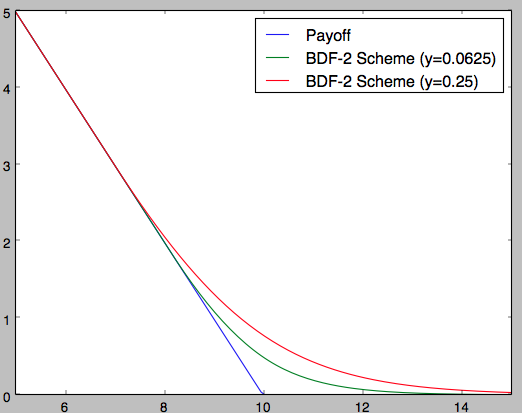
\includegraphics[width=0.6\textwidth]{img/Heston_price.png}
\end{figure}


%%---------------- APPENDIX ----------------%%

\newpage
\section{Appendix}

	\subsection{Proofs of section 1}
	
		\subsubsection{Consistency of BDF-2}

Using Taylor's theorem we have the following inequalities,
\begin{align*}
\abs{ \frac{u_{j+1}^{n+1}-u_{j-1}^{n+1}}{2h} - u_x(t_{n+1},x_j) } \leq \frac{h^2}{9} \ninf{u_{3x}}, \\
\abs{ \frac{u_{j+1}^{n+1}-2u_{j}^{n+1}+u_{j-1}^{n+1}}{2h} - u_{xx}(t_{n+1},x_j) } \leq \frac{h^2}{12} \ninf{u_{4x}}, \\
\abs{ \frac{3u_{j}^{n+1} - 4u_{j}^{n} + u_{j}^{n-1}}{2 \tau} - u_t(t_{n+1},x_j) } \leq \frac{2 \tau^2}{3} \ninf{u_{3t}},
\end{align*}
and since the obstacle term is at $t_{n+1}$ in (\ref{eq-BDF2}), the scheme is second order consistent in time and space.

		\subsubsection{Consistency of BDF-3}

The result is straighforward from the proof of the consistency of BDF-2 and the additionnal inequality obtained using Taylor's theorem,
\begin{align*}
\abs{ \frac{\frac{11}{6} u_j^{n+1} - 3 u_j^n + \frac{3}{2} u_j^{n-1} - \frac{1}{3} u_j^{n-2}}{\tau} - u_t(t_{n+1},x_j) } \leq \frac{\tau^3}{4} \ninf{u_{4t}}.
\end{align*}


\newpage
\bibliographystyle{plain}
\bibliography{biblio}

\end{document}